\documentclass[10pt,a4paper]{report}
\usepackage{cmap}
\usepackage[russian]{babel}
\usepackage{amsmath}
\usepackage{amsfonts}
\usepackage{amssymb}
\usepackage{graphicx}
\graphicspath{{image/}}
\usepackage{listings}
\usepackage{hyperref}
\usepackage{float}
\usepackage{fontspec}
\setmainfont{Times New Roman}
\setmonofont{Arial}

\lstset{
	inputencoding=utf8x,
	extendedchars=\true,
	frame=single,
	breaklines=true,
	numbers=left,
	keepspaces = true}

\voffset -24.5mm
\hoffset -5mm
\textwidth 173mm
\textheight 240mm
\oddsidemargin=0mm \evensidemargin=0mm

\author{Абдуллин Азат}
\title{Руководство программиста}
\begin{document}
\maketitle
\renewcommand{\thesection}{\arabic{section}}
\tableofcontents
\pagebreak
	
\section{Назначение и условия применения программы}
Данная программа предназначена для запуска графических пользовательских приложений 	в ОС Linux на платформе Raspberry Pi Zero. Для запуска программы в системе должны быть установлены пакеты Wayland и WLC.
		
\section{Обращение к программе}
Программа имеет один входной параметр --- путь к конфигурационному файлу. При отсутствии данного аргумента программа открывает файл по-умолчанию \texttt{~/.config/xxwm}. При запуске оконного менеджера автоматически запускаются системные приложения строки состояния и рабочего стола. Имеется возможность указания исполняемых файлов системных приложений в конфигурационном файле. Формат конфигурационного файа приведен в листинге \ref{lst:conf}
\begin{lstlisting}[label=lst:conf, caption={Формат конфигурационного файла}]
[statusbar]
exe=*path to executable*

[desktop]
exe=*path to executable*
\end{lstlisting}

При запуске программы на экране отображается строка состояния и рабочий стол (рис. \ref{fig:wm1}).
\begin{figure}[h!]
\center{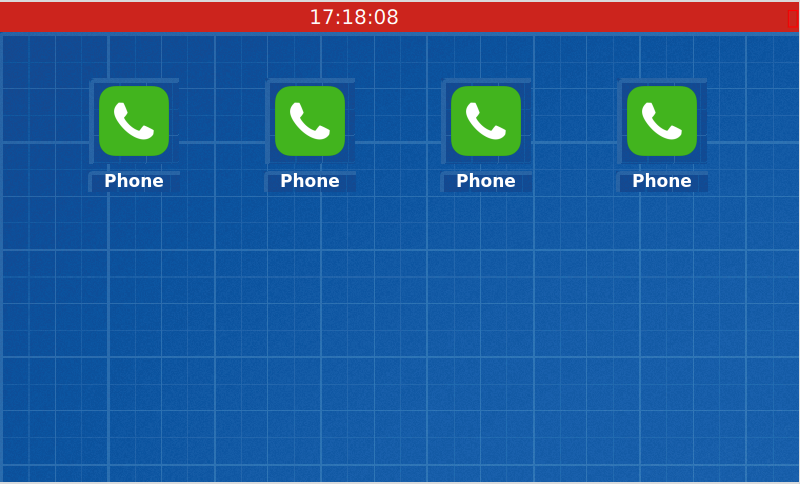
\includegraphics[width=\linewidth]{wm1}}
\caption{Стартовый вид программы}
\label{fig:wm1}
\end{figure}

При нажатии на одну из иконок на рабочем столе запустится соответствующее приложение (рис. \ref{fig:wm5}).
\begin{figure}[h!]
\center{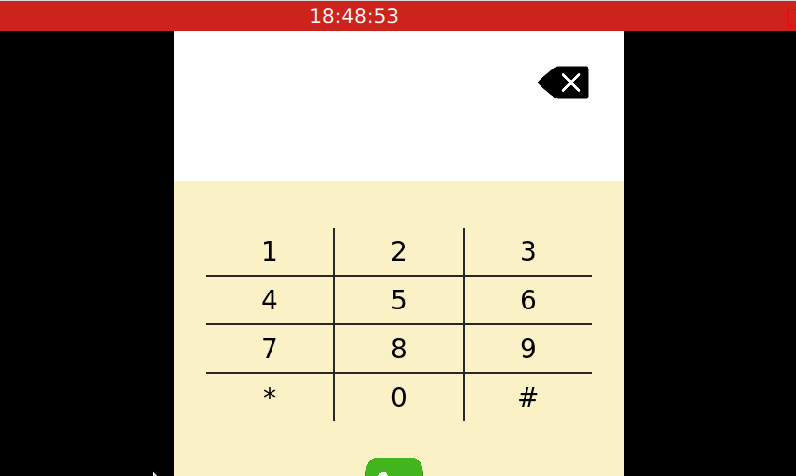
\includegraphics[width=\linewidth]{wm5}}
\caption{Запуск приложения с рабочего стола}
\label{fig:wm5}
\end{figure}

Программа поддерживает следующие комбинации клавиш:
\begin{itemize}
\item CTRL+Enter --- запуск терминала (рис. \ref{fig:wm2})
\item CTRL+q --- закрытие приложения
\item CTRL+стрелка вниз --- переключение окон
\item CTRL+Esc --- завершение работы программы
\end{itemize}
\begin{figure}[h!]
\center{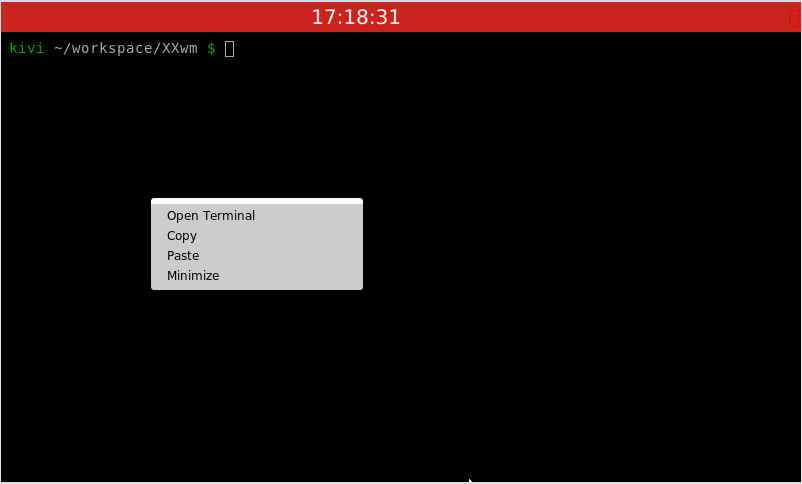
\includegraphics[width=\linewidth]{wm2}}
\caption{Запуск терминала}
\label{fig:wm2}
\end{figure}

Программа так же поддерживает управление окнами с помощью мыши (рис. \ref{fig:wm4}):
\begin{itemize}
\item CTRL+ЛКМ --- перемещение окна
\item CTRL+ПКМ --- изменение размеров окна
\end{itemize}
\begin{figure}[h!]
\center{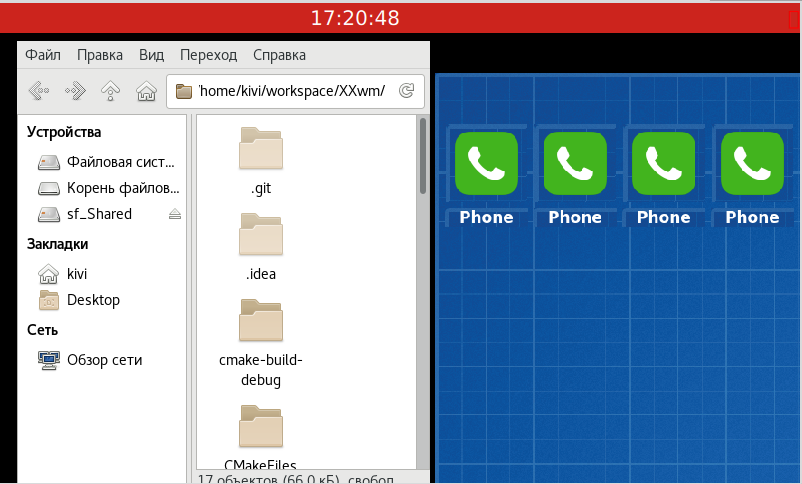
\includegraphics[width=\linewidth]{wm4}}
\caption{Управление окнами с помощью мыши}
\label{fig:wm4}
\end{figure}

\section{Структура программы}
Структурно программный комплекс делится на две подсистемы: подсистема считывания конфигурации и оконный менеджер.
		
\subsection{Подсистема считывания конфигурации}
Данная подсистема необходима для считывания конфигурационного файла и определения параметров запуска оконного менеджера. Подсистема состоит из двух файлов:
\begin{itemize}
\item config.h --- заголовочный файл с определениями функций
\item config.c --- файл с реализациями функций
\end{itemize}

Система считывания конфигурации содержит следующие функции:
\begin{itemize}
\item \texttt{init\_config} --- функция инициализация конфигурации. В качестве входного параметра необходимо передать имя файла конфигурации в виде строки. Выходные параметры отсутствуют.
\item \texttt{get\_statusbar} --- функция считывает имя исполняемого файла строки состояния. Перед вызовом конфигурация должна быть проинициализирована вызовом функции \texttt{init\_config}. Входные параметры отсутствуют. Выходной параметр --- имя исполняемого файла строки состояния в виде строки.
\item \texttt{get\_desktop} --- функция считывает имя исполняемого файла рабочего стола. Перед вызовом конфигурация должна быть проинициализирована вызовом функции \texttt{init\_config}. Входные параметры отсутствуют. Выходной параметр --- имя исполняемого файла рабочего стола в виде строки.
\end{itemize}

Так же содержится переменная \texttt{configuration} --- структура, которая хранит считанную конфигурацию. Устанавливается в функции \texttt{init\_config}.

\subsection{Подсистема <<Оконный менеджер>>}
Данная реализует функции оконного менеджера и отвечает за его запуск. Подсистема состоит из файла main.c.
Оконный менеджер содержит следующие функции:
\begin{itemize}
\item \texttt{start\_interactive\_action} --- функция которая начинает интерактивное действие. Входные параметры:
	\begin{itemize}
	\item идентификатор окна, на котором начинается действие
	\item точка, в которой начато действие
	\end{itemize}
	
Выходные параметры: \texttt{true} если действие было начато, иначе \texttt{false}.

\item \texttt{start\_interactive\_move} --- функция, которая начинает интерактивное действие передвижения окна. Входные параметры:
	\begin{itemize}
	\item идентификатор окна, на котором начинается действие
	\item точка, в которой начато действие
	\end{itemize}
	
Выходные параметры отсутствуют.

\item \texttt{start\_interactive\_resize} --- функция, которая начинает интерактивное действие изменения размеров окна. Входные параметры:
	\begin{itemize}
	\item идентификатор окна, на котором начинается действие
	\item грань окна, которая должна быть передвинута
	\item точка, в которой начато действие
	\end{itemize}
	
Выходные параметры отсутствуют.

\item \texttt{stop\_interactive\_action} --- функция, которая завершает интерактивное действие. Входные параметры отсутствуют. Выходные параметры отсутствуют.

\item \texttt{get\_topmost} --- функция получения окна по смещению.  Входные параметры:
	\begin{itemize}
	\item идентификатор отображаемого экрана
	\item смещение
	\end{itemize}
	
	Выходной параметр --- идентификатор окна.

\item \texttt{relayout} --- функция перерисовывания экрана.  Входные параметры:
	\begin{itemize}
	\item идентификатор отображаемого экрана
	\end{itemize}
	
	Выходные параметры отсутствуют.
	
\item \texttt{output\_resolution} --- функция смены разрешения экрана.  Входные параметры:
	\begin{itemize}
	\item идентификатор отображаемого экрана
	\item старое разрешение
	\item новое разрешение
	\end{itemize}
	
	Выходные параметры отсутствуют.
	
\item \texttt{view\_created} --- функция обработки отображения нового окна.  Входные параметры:
	\begin{itemize}
	\item идентификатор окна
	\end{itemize}
	
	Выходной параметр: \texttt{true} если окно обработано, \texttt{false} если окно необходимо уничтожить.
	
\item \texttt{view\_destroyed} --- функция обработки уничтожения окна.  Входные параметры:
	\begin{itemize}
	\item идентификатор окна
	\end{itemize}
	
	Выходные параметры отсутствуют.
	
\item \texttt{view\_focus} --- функция установки активного окна.  Входные параметры:
	\begin{itemize}
	\item идентификатор окна
	\item \texttt{true} если окно необходимо сделать активным
	\end{itemize}
	
	Выходные параметры отсутствуют.
	
\item \texttt{view\_request\_move} --- функция запроса перемещения окна.  Входные параметры:
	\begin{itemize}
	\item идентификатор окна
	\item координаты начального положения окна
	\end{itemize}
	
	Выходные параметры отсутствуют.
	
\item \texttt{view\_request\_resize} --- функция запроса изменения размера окна.  Входные параметры:
	\begin{itemize}
	\item идентификатор окна
	\item грань окна, которая должна быть передвинута
	\item координаты начального положения окна
	\end{itemize}
	
	Выходные параметры отсутствуют.
	
\item \texttt{view\_request\_geometry} --- функция запроса изменения параметров отображения окна.  Входные параметры:
	\begin{itemize}
	\item идентификатор окна
	\item новые параметры отображения окна
	\end{itemize}
	
	Выходные параметры отсутствуют.
	
\item \texttt{keyboard\_key} --- функция обработки клавиш клавиатуры.  Входные параметры:
	\begin{itemize}
	\item идентификатор окна
	\item время нажатия
	\item флаги модификаторов клавиатуры
	\item код клавиши
	\item состояние клавиши
	\end{itemize}
	
	Выходной параметр: \texttt{false} если событие необходимо передать окну.
	
\item \texttt{pointer\_button} --- функция обработки кнопок мыши.  Входные параметры:
	\begin{itemize}
	\item идентификатор окна
	\item время нажатия
	\item флаги модификаторов клавиатуры
	\item код кнопки
	\item состояние кнопки
	\item позиция указателя мыши
	\end{itemize}
	
	Выходной параметр: \texttt{false} если событие необходимо передать окну.
	
\item \texttt{pointer\_motion} --- функция обработки перемещения указателя мыши.  Входные параметры:
	\begin{itemize}
	\item идентификатор окна
	\item время перемещения
	\item позиция указателя мыши
	\end{itemize}
	
	Выходной параметр: \texttt{false} если событие необходимо передать окну.
	
\item \texttt{cb\_log} --- функция логирования.  Входные параметры:
	\begin{itemize}
	\item тип сообщения
	\item сообщение
	\end{itemize}
	
	Выходные параметры отсутствуют.
\end{itemize}

Так же содержится переменная \texttt{compositor} --- структура, которая хранит информацию об интерактивном действии. Используется в функциях обработки интерактивных действий.

\section{Установка и настройка программы}
\subsection{Состав установочного комплекта}
\begin{itemize}
\item main.c --- основной файл оконного менеджера
\item config.h --- заголовочный файл с объявлениями функций считывания конфигурации
\item config.c --- файл с определениями функций считывания конфигурации
\item CMakeLists.txt --- файл сборки программы
\item config.ini --- файл конфигурации
\item xxon.desktop --- файл ярлыка для экранного менеджера
\end{itemize}

\subsection{Установка программы}
Первым шагом при подготовке оконного менеджера к работе является компиляция исходных кодов программы в бинарные файлы. Для компиляции необходимо воспользоваться системой сборки CMake, версии, не ниже 3.7. Так же в системе должны быть установлены компилятор GCC и система сборки Make.
Компиляция осуществляется следующими командами:
\begin{verbatim}
cmake .
make
\end{verbatim}
В результате, в рабочей директории появится исполняемый файл оконного менеджера xxwm.
					
Для установки программы необходимо иметь права администратора. Для установки необходимо:
\begin{itemize}
\item Поместить исполняемый файл оконного менеджера в каталог исполняемых файлов:
\begin{verbatim}
cp xxwm /usr/bin/
\end{verbatim}
\item Поместить стандартный конфигурационный файл в директорию хранения конфигураций:
\begin{verbatim}
cp config.ini ~/.config/xxwm
\end{verbatim}
\item Поместить файл ярлыка для экранного менеджера в директорию ярлыков оконных менеджеров:
\begin{verbatim}
cp xxon.desktop /usr/share/wayland-sessions/
\end{verbatim}
\end{itemize}

\subsection{Настройка программы}
Для настройки программы необходимо в конфигурационном файле ~/.config/xxwm указать пути к исполняемым файлам строки состояния и рабочего стола
				
\subsection{Деинсталяция программы}
Для деинсталляции программы необходимо удалить ранее скопированные файлы:
\begin{verbatim}
rm /usr/bin/xxwm
rm ~/.config/xxwm
rm /usr/share/wayland-sessions/xxon.desktop
\end{verbatim}

\section{Проверка программы}
Методики проверки работоспособности программы описаны в документе "Программа и методика испытаний".
			 
\end{document}